\section{Background modelling}

\textbf{Pre-fit distributions}

I think this is a great place to show the unrolled plots year-by-year. (I might try to overlay the postfit plots in the next step though). 


\begin{itemize}
	\item Background systs uncorrelated across the years, but correlated across the \Xhh and \deta cats within a year
	\item VBF fits all of the years together
\end{itemize}

\subsection{B-only fits (?)}

Post-fit (ggF) background only fits:

\def\figDir{figures/nr-int-note/unblind_results/V6/}
\foreach \yr in {16,17,18}{
    \begin{figure}[htp]
    	\centering
    	\includegraphics[width=.32\textwidth]{\figDir/postfit-plot-correlated-fullsyst-unblind-bkg-new-deta-Xhh-3x2-res-p09-ggf-\yr-dEta-1-Xhh-1} 
    	\includegraphics[width=.32\textwidth]{\figDir/postfit-plot-correlated-fullsyst-unblind-bkg-new-deta-Xhh-3x2-res-p09-ggf-\yr-dEta-2-Xhh-1} 
    	\includegraphics[width=.32\textwidth]{\figDir/postfit-plot-correlated-fullsyst-unblind-bkg-new-deta-Xhh-3x2-res-p09-ggf-\yr-dEta-3-Xhh-1} \\
	\includegraphics[width=.32\textwidth]{\figDir/postfit-plot-correlated-fullsyst-unblind-bkg-new-deta-Xhh-3x2-res-p09-ggf-\yr-dEta-1-Xhh-2} 
    	\includegraphics[width=.32\textwidth]{\figDir/postfit-plot-correlated-fullsyst-unblind-bkg-new-deta-Xhh-3x2-res-p09-ggf-\yr-dEta-2-Xhh-2} 
    	\includegraphics[width=.32\textwidth]{\figDir/postfit-plot-correlated-fullsyst-unblind-bkg-new-deta-Xhh-3x2-res-p09-ggf-\yr-dEta-3-Xhh-2} \\
    	\caption{ggF 20\yr \ background only post-fit plots.}
    	\label{fig:ggf-postfit-\yr}
    \end{figure}
}

\textbf{Q: Do I also have the unrolled post-fit plots in the folder?}
%\begin{figure}[htp]
%\centering
%	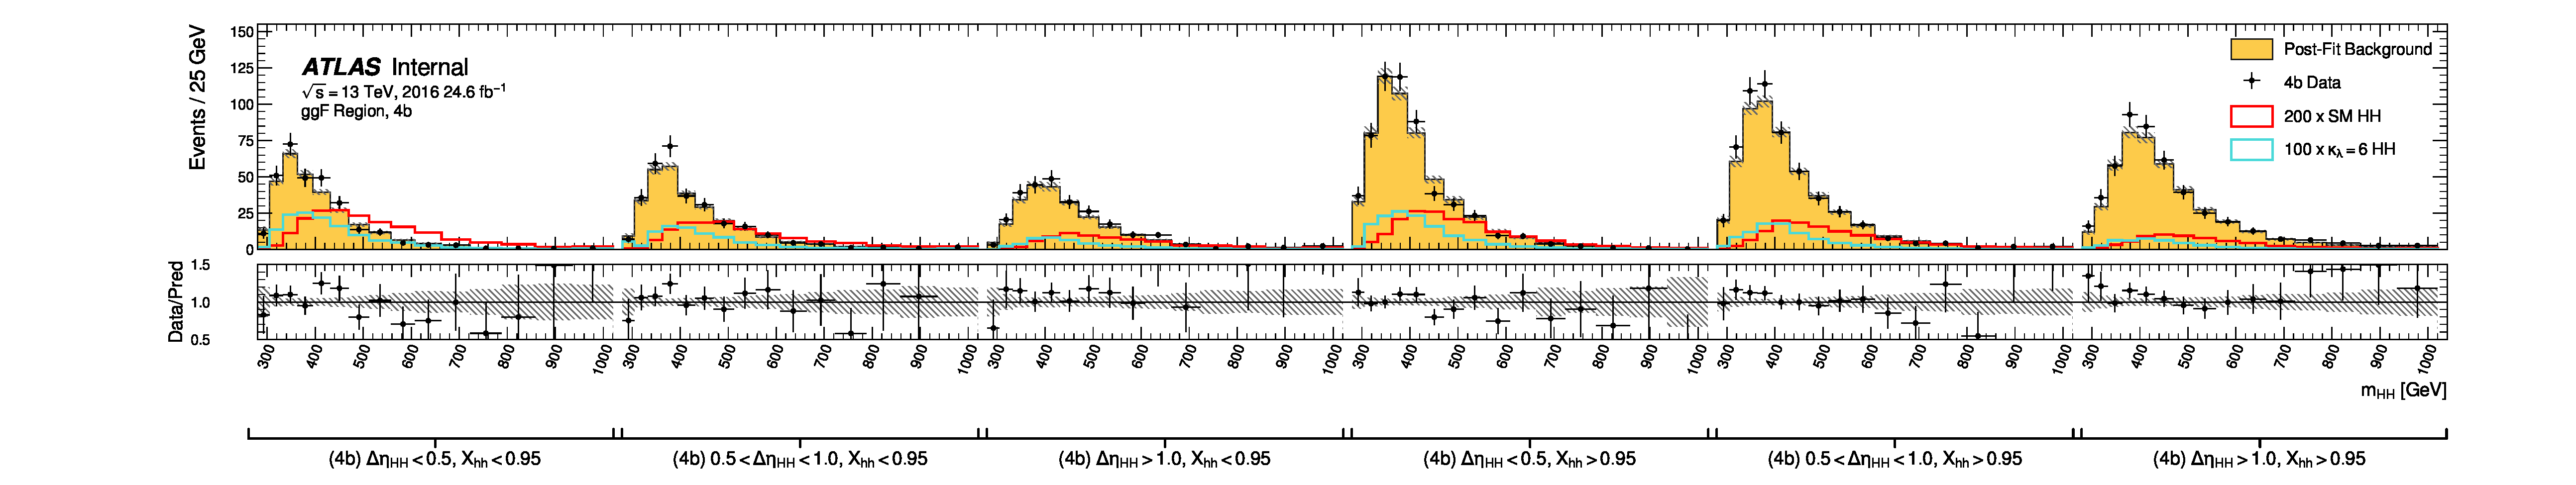
\includegraphics[width=\textwidth]{unrolled_postfit-plot_correlated_fullsyst_unblind_bkg_new_deta_Xhh_3x2_res_p09_ggf_16} \\
%	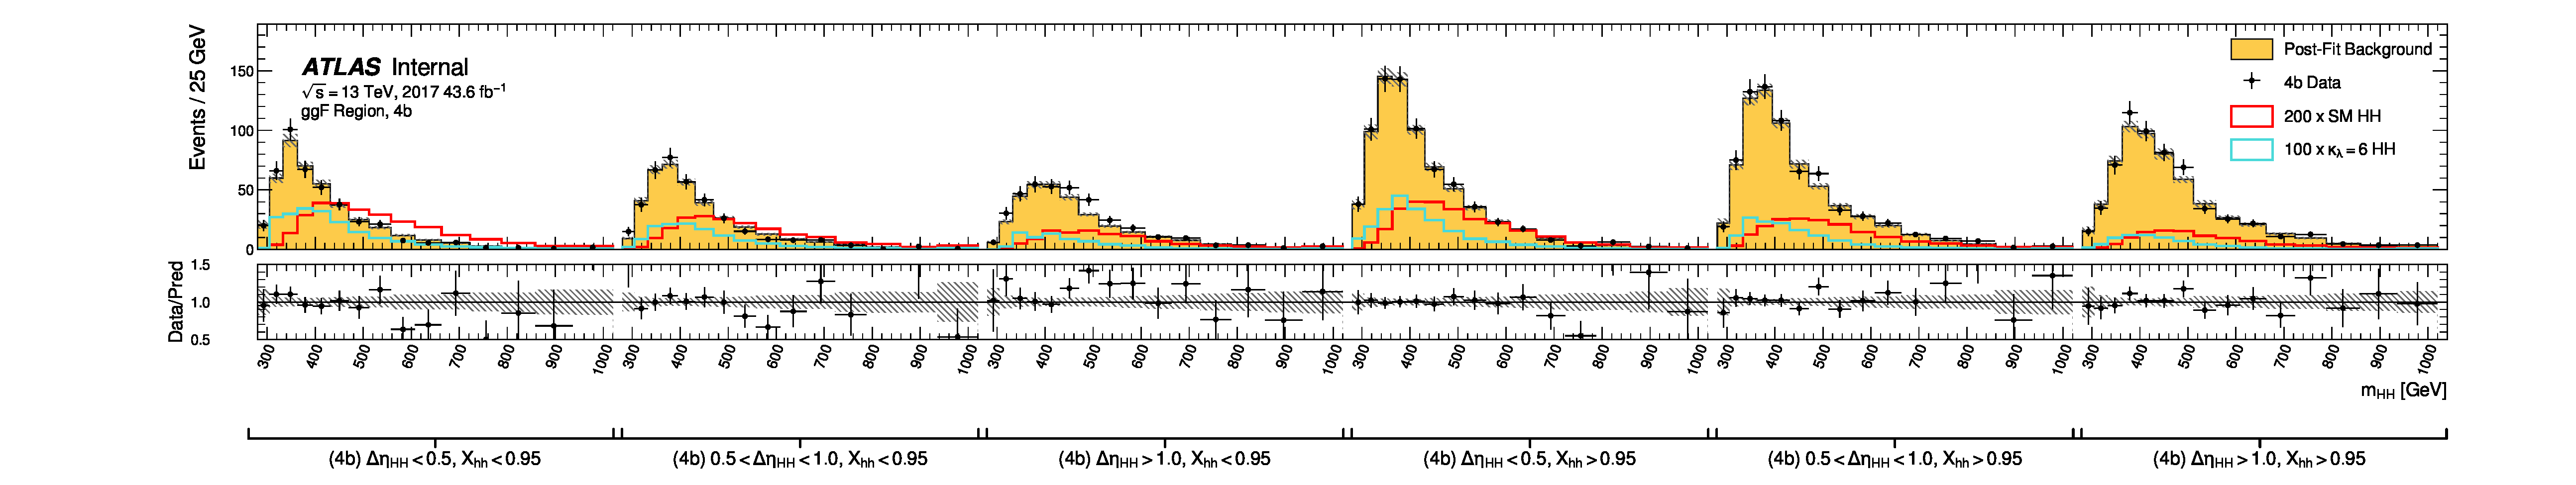
\includegraphics[width=\textwidth]{unrolled_postfit-plot_correlated_fullsyst_unblind_bkg_new_deta_Xhh_3x2_res_p09_ggf_17} \\
%	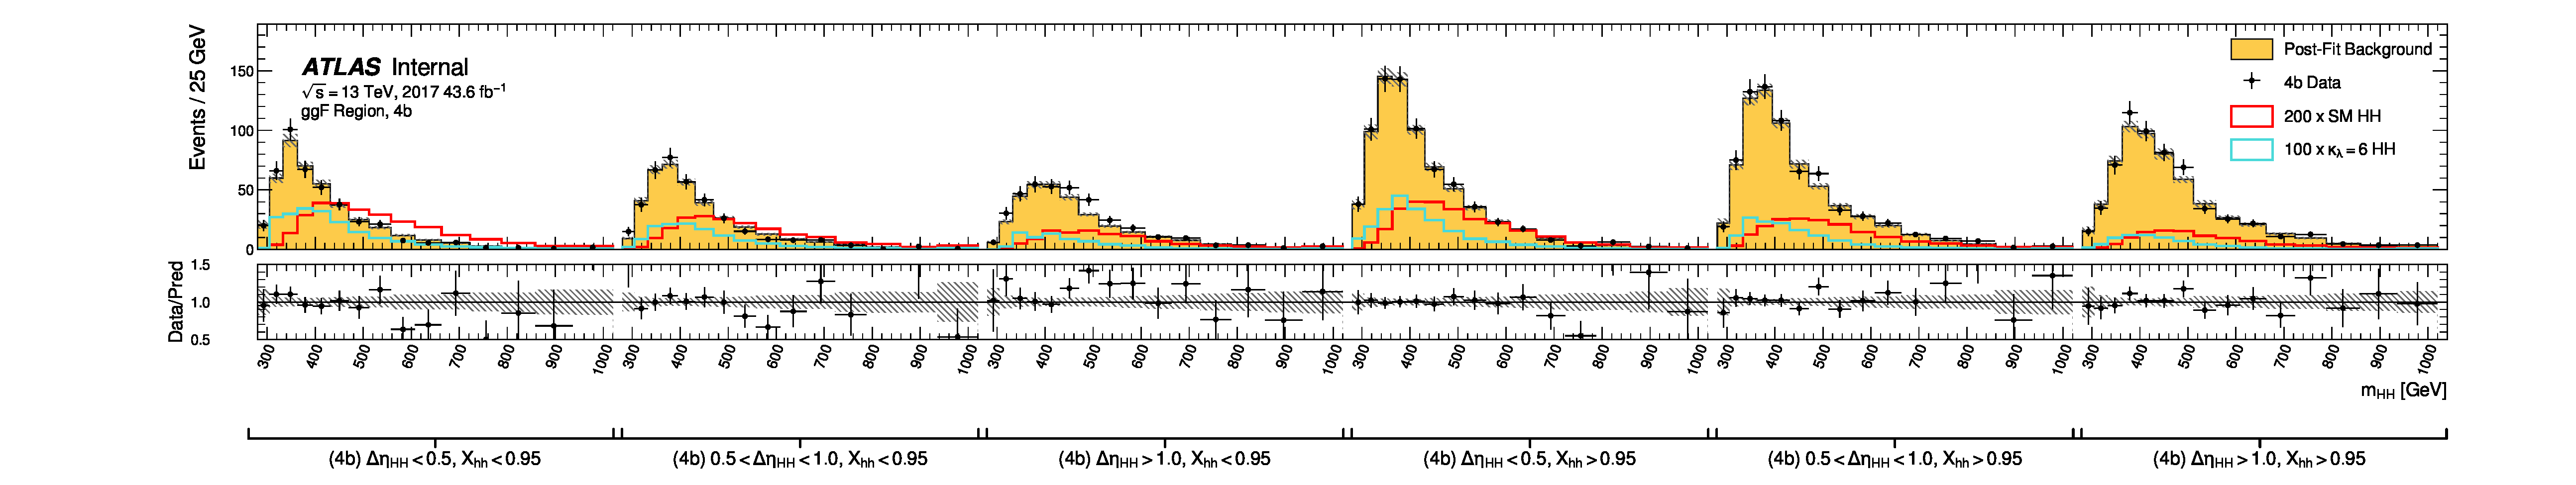
\includegraphics[width=\textwidth]{unrolled_postfit-plot_correlated_fullsyst_unblind_bkg_new_deta_Xhh_3x2_res_p09_ggf_17}
%	\caption{ggF postfit plots.}
%	\label{fig:ggf-postfit}
%\end{figure}


\textcolor{red}{
New organization ideas: 
\begin{itemize}
\item I want to over pre and post-fit \emph{just with unrolled plots} to quantify the non-closure.
\item Then for the plots that also overlay the signals, I will put all of the years on top of each other.
\end{itemize}
}

The NP pulls are shown in \Fig{\ref{fig:ggf-pulls-corr-bonly}}.
No large constraints are observed.
Some pulls from some components are expected due to the transition from CR to SR.
Especially $Q_E$ and $Q_S$ in 2016 ggF provide shape variations that particularly impact the \mhh peak (see top left plot in \Fig{\ref{fig:sr-np-impact-by-cat}}), therefore they are the most pulled.
For the background estimation uncertainties, the nuisance parameter naming scheme is alpha\_\{syst\}\_\{quad\}\_\{year\}.
For example `alpha\_CR12\_shape\_N\_ggf\_16' stands for `CR12 shape uncertainty North quad in 2016'.
Note that `Non-Closure 3b1f' doesn't have a split in quadrants.
From a S+B fit, a correlation matrix is derived and shown in \Fig{\ref{fig:ggf-correlation-matrix-corr-sm}}.

\noindent{VBF cat only fits}

Similar to the ggF channel, the background shape systematics (CR12) are treated as correlated across \deta bins in the VBF channel.
Since we derive the VBF background estimate with the years inclusively and do the fits inclusively, we do not have separate background NPs for each year in the VBF channel.

The post-fit VBF plots in the $\Delta \eta_{HH}$ categories are shown in \Fig{\ref{fig:vbf-postfit}}.

\begin{figure}[htp]
\centering
	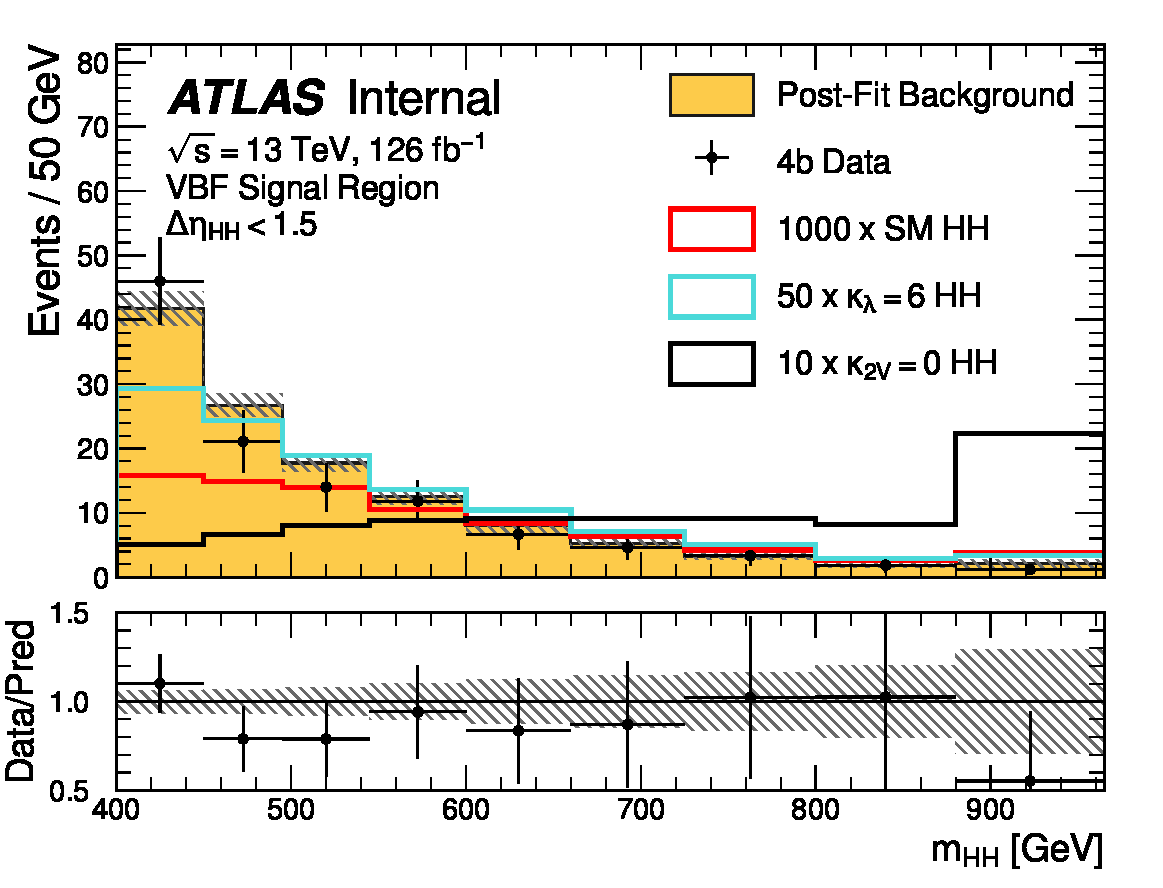
\includegraphics[width=.44\textwidth]{\figDir/postfit-plot-correlated-fullsyst-unblind-vbf-only-deta-2-cats-noggF-vbf--1-dEta-1} 
	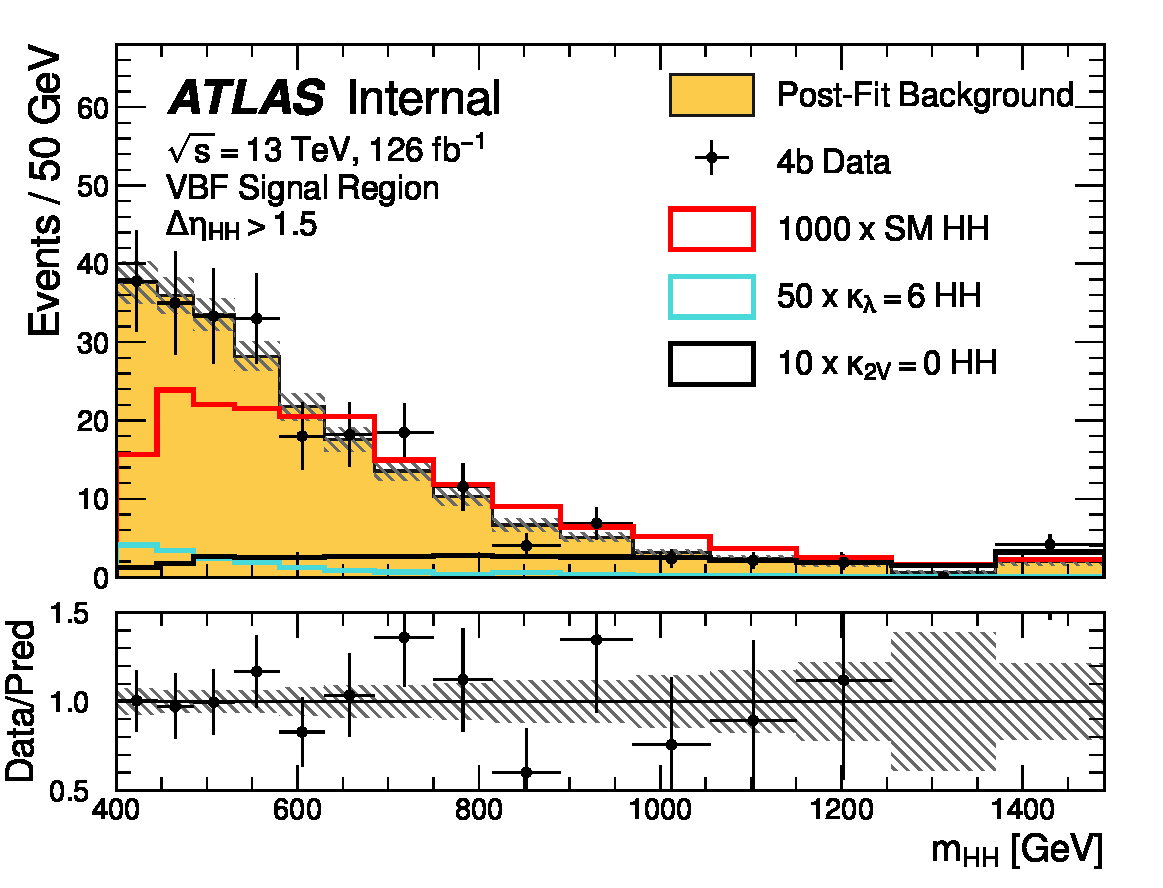
\includegraphics[width=.44\textwidth]{\figDir/postfit-plot-correlated-fullsyst-unblind-vbf-only-deta-2-cats-noggF-vbf--1-dEta-2} 
	\caption{VBF background only post-fit plots.}
	\label{fig:vbf-postfit}
\end{figure}

